\chapter{Stability of the river banks}
\section{River bank instability due to sand mining}
Much like the Paraná Guazú, sand mining is a relevant topic in the lower Mekong river. Previous studies have shown that incision due to the sand mining exists in this river and is of the order of 0.13 m per year \autocite{brunierRecentMorphologicalChanges2014}. \citeauthor{hackneyRiverBankInstability2020} showed that this river bed lowering not only has morphological consequences but also geotechnical ones, since a lower river bed can cause instability of the river banks.

In the previous study it was found that, even in conservative scenarios, entire sections of river banks along the lower Mekong River would shift from a stable to a seasonally unstable condition. This means they are likely to fail during periods of heavy rainfall. In more extreme scenarios with more sand mining, the researchers found that 63\% of river banks would become seasonally unstable \autocite{hackneyIncreasedHydraulicRoughness2025}.

In this chapter, the potential risks of river bank instability due to sand mining in the Paraná Guazú-river are investigated.

\section{Geological background}
To understand more about bank erosion, one first must have knowledge of the soil profile in the delta region. This section intends to combine all the available information regarding the subsoil in the investigation area.

\subsection{The geology of a delta}
A delta is a landscape formed at the mouth of a river where the water eventually runs into the ocean. At a delta, the water's velocity decreases which gives floating particles in the delta the change to settle. Among these floating particles are gravels, sands and clays, descending in particle size. The particles are formed by erosion of stone. The origin of the particles in the Parana river are the Andes mountains. 
Besides that, deltas are also characterized by high vegetation growth. When this vegetation dies, the organic material will change into peat due to the governing pressures. So, in a delta one expects to find relatively soft soils (sands) and very soft soils (clay and peat).

\subsection{Geological cross sections}
A study by \citeauthor{joseluiscavallottoEvolucionCambiosAmbientales2005} was conducted that led to a morphological map of the Paraná delta. In the study, for two cross sections a more detailed geological profile was made, one of which is relevant to the area of interest. The cross section along with the area of interest is shown in figure \ref{fig:crosssectiongeo}.

\begin{figure}[H]
    \centering
    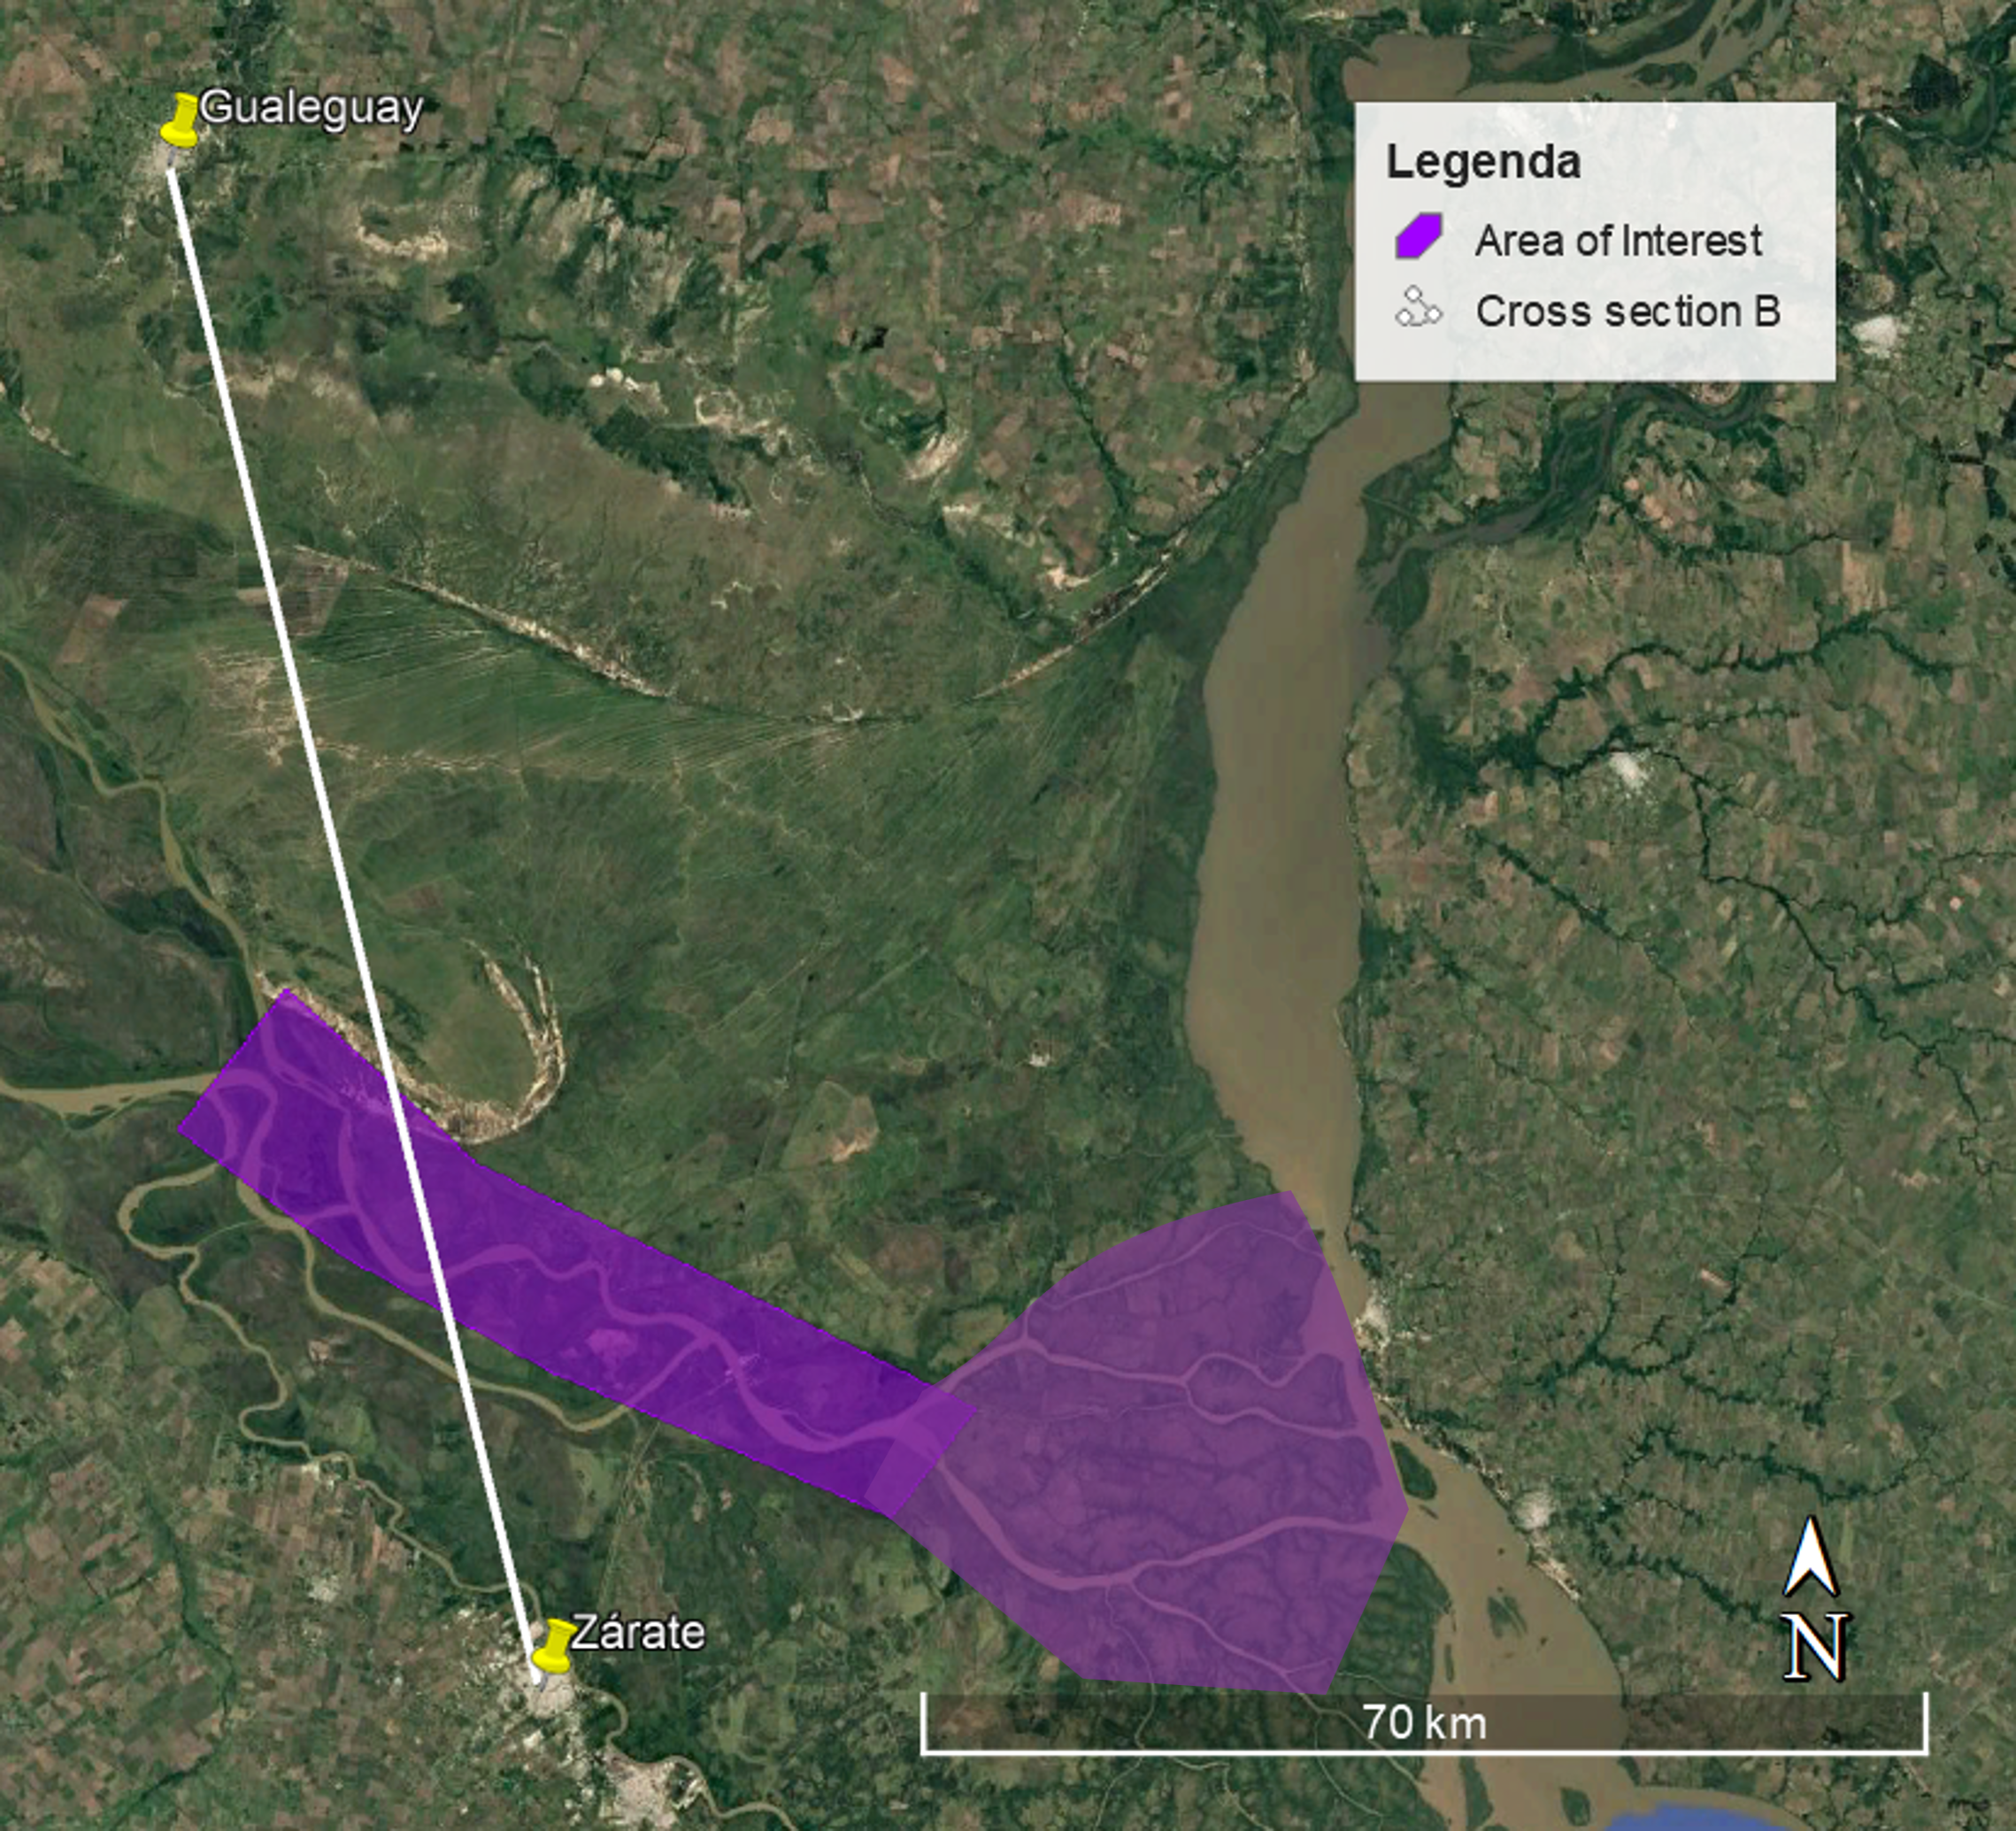
\includegraphics[width=0.75\linewidth]{figures/ch9/CrossSectionB.png}
    \caption{Cross section}
    \label{fig:crosssectiongeo}
\end{figure}

The geological profile of the cross section is shown in figure \ref{fig:geolprofile}. As can be seen in the figure, the taken cross section was around 80 km long. Of this, 15 km falls inside the area of interest, this zone is marked with purple.

\begin{figure}[H]
    \centering
    \includegraphics[width=1\linewidth]{figures/ch9/CrossSectionBResults.png}
    \caption{Geological profile of cross section \autocite{joseluiscavallottoEvolucionCambiosAmbientales2005}}
    \label{fig:geolprofile}
\end{figure}

In figure \ref{fig:geolprofile}, the first kilometers of the purple zone are especially of interest since these are located near the river. The following layers can be identified in this area.

\subsubsection{Subaerial facies}
The subaerial facies of the Paraná Delta developed through the deposition of silty-sandy sediments delivered mainly by the Paraná Guazú and Paraná de las Palmas \autocite{joseluiscavallottoEvolucionCambiosAmbientales2005}. These deposits occur at elevations between 2 m and sea level, with a maximum thickness of 12 m. This is the layer that is drained.

Mineralogical analyses show a predominance of quartz with minor plagioclase and K-feldspar, plus heavy minerals such as magnetite, hematite, garnet, zircon, tourmaline, and others, generally well-rounded except zircon, which preserves crystal form \autocite{rafaelcordiniContribucionConocimientoGeologia1949}. The age of the unit is debated: radiocarbon dates suggest origin dates between -150 BC and 180 AD, while other authors propose a later origin around 700–750 AD \autocite{joseluiscavallottoEvolucionCambiosAmbientales2005}.

\subsubsection{Open estuary}
The open estuary sediments were deposited during postglacial sea-level rise and were formed at the freshwater–saltwater interface during the upstream migration of the maximum salinity gradient, which filled the Río de la Plata river valley \autocite{joseluiscavallottoEvolucionCambiosAmbientales2005}.

These are olive-green clays to silty clays with thin fine-sand layers, scattered or concentrated shell beds, and fossil content confirming estuarine conditions. The unit is dated to the Holocene, with its base at ~6670 +/- 100 years BC, occurring between –22 and –0 m and reaching up to 20 m thick \autocite{vogelGroningenRadiocarbonDates1969}.

\subsubsection{Paranense depositional sequence}
During the Miocene, large portions of present-day Argentina, Uruguay, Paraguay, southern Brazil, and eastern Bolivia were covered by the Paranense Sea. This was a shallow sea that advanced from the Atlantic into the interior of South America . Its waters left behind extensive marine sediments and fossils and this layer is now known as the Paranense depositional sequence \autocite{tineoReconstructingSouthAmerican2024}.

It is composed mainly of siliciclastic sandstones, mudstones, and bioclastic beds, with thicknesses ranging from a few meters in outcrop to over 100 m. The lower part has mud-dominated offshore deposits with marine fossils, while the upper part shows sandier shoreface. Studies constrain the unit to the Late Miocene (ca. 9.5–6.7 Ma) \autocite{tineoReconstructingSouthAmerican2024}.

\subsubsection{Cross section by \citeauthor{amatoESTRATIGRAFIACUATERNARIASUBSUELO2009}}
Another study focuses on subsurface deposits from Diamante in Entre Ríos to San Fernando in the Buenos Aires province. Based on lithologic, clay mineral, radiocarbon, and outcrop data, the authors propose a depositional model for the region. This geological cross section is shown in figure \ref{fig:depmodel}. The purple area marks the area of interest for this research (Puerto Ibicuy).

\begin{figure}
    \centering
    \includegraphics[width=1\linewidth]{figures/ch9/Crosssection2.png}
    \caption{Depositional model \autocite{amatoESTRATIGRAFIACUATERNARIASUBSUELO2009}}
    \label{fig:depmodel}
\end{figure}

As can be seen in the figure, the first layer consists of deltaic and flooplain deposits from the Holocene until recent times. This is in accordance with the geological profile as shown in figure \ref{fig:crosssectiongeo}. Underneath, holocene coastal/estuarine sediments can be found and below there are the Plio–Pleistocene fluvial deposits. The estuarine sediments can also be found in figure \ref{fig:crosssectiongeo}, but a different conclusion was reached for the final layer. \citeauthor{joseluiscavallottoEvolucionCambiosAmbientales2005} conclude that this is a pre-holocene marine deposit from the Miocene Paranense Sea, while here Plio–Pleistocene river deposits are placed below the Holocene sequence.

\section{Borehole}
In the same study conducted by \citeauthor{amatoESTRATIGRAFIACUATERNARIASUBSUELO2009}, a number of boreholes were executed along the lower Paraná \autocite{amatoESTRATIGRAFIACUATERNARIASUBSUELO2009}. One of these boreholes were executed near the area of interest in Puerto Ibicuy. The borehole was interpreted and with this the following soil profile was made  \autocite{amatoESTRATIGRAFIACUATERNARIASUBSUELO2009}.

\begin{figure}[H]
    \centering
    \includegraphics[width=0.45\linewidth]{figures//ch9/Bodemprofiel.png}
    \caption{Borehole profile in Puerto Ibicuy}
    \label{fig:borehole}
\end{figure}

\section{Geotechnical summary}
To get an overview of possible river bank instability, the soil layers along with their geotechnical parameters should be known. For this, the borehole is deemed the most relevant source. The borehole shows a top layer with fine/medium sands. Below, clay/clayey sand can be found, and the bottom layer consists of medium sand. This is in accordance with the geological profiles that were provided before in figures \ref{fig:crosssectiongeo} and \ref{fig:depmodel}. Both frameworks describe a fluvial-to-estuarine-to-marine vertical transition. The top fluvial deposits help declare the presence of sandy deposits at the top and the layers of clay/clayey sand below correspond to estuarine deposits. Finally, old marine/fluvial deposits were likely compacted and lead to the layer of medium sand found at the bottom of the borehole.

Because of the resemblance between the local borehole and geological profiles given before, the layering as shown in figure \ref{fig:borehole} is deemed representative for the whole study area. Based on this layering the relevant parameters can be derived, the result in shown in table \ref{tab:soil_layers}.

\begin{table}[H]
    \centering
    \begin{tabular}{|c|c|c|c|c|c|c|c|}
        \hline
        Start layer (m) & End layer (m) & Soil type & \makecell{ $\gamma_d$ \\ (kN/m$^3$) } & \makecell{ $\gamma_{sat}$ \\ (kN/m$^3$) } & \makecell{ $\varphi'$ \\ ($^\circ$) } & \makecell{ $c'$ \\ (kPa) } & \makecell{ $c_u$ \\ (kPa) } \\
        \hline
        0 & 2 & Fill (Topsoil/Agricultural) & 12 & 12 & 15 & 2.5 & 20 \\
        2 & 7 & Fine/medium sand & 17 & 19 & 30 & 0 & - \\
        7 & 10 & Clay & 14 & 14 & 17.5 & 0 & 25 \\
        10 & 15 & Clayey sand & 18 & 20 & 25 & 0 & - \\
        15 & 16 & Clay & 14 & 14 & 17.5 & 0 & 25 \\
        16 & 17.5 & Clayey sand & 18 & 20 & 25 & 0 & - \\
        17.5 & 32 & Medium sand & 18 & 20 & 32.5 & 0 & - \\
        \hline
    \end{tabular}
    \caption{Soil stratigraphy and geotechnical properties.}
    \label{tab:soil_layers}
\end{table}

The parameters in table \ref{tab:soil_layers} were derived from the Eurocode (

TOp layer not named, assumed organic topsoil
“Parameters for fill are assumed based on typical values for organic topsoil; actual values to be confirmed by laboratory testing.”